\documentclass[12pt, a4paper, lithuanian, final]{article}

\usepackage{hyperref}
\usepackage{graphicx}
\usepackage{float}
\usepackage{placeins}
\usepackage{gensymb}
\usepackage{xcolor}
\usepackage{listings}
\usepackage{amsmath}
\usepackage{textgreek}
\usepackage{mathtools}
\usepackage[obeyFinal]{easy-todo}
\usepackage[utf8]{inputenc}
\def\LTfontencoding{L7x}
\usepackage[\LTfontencoding]{fontenc}
\usepackage[lithuanian]{babel}
%\usepackage{times}

%\renewcommand{\sfdefault}{uhv}
%\renewcommand{\rmdefault}{utm}
%\renewcommand{\ttdefault}{ucr}

\usepackage{VUMIF}

%Kodo highlitinimo configas
\lstset{basicstyle=\ttfamily,
	showstringspaces=false,
	commentstyle=\color{red},
	keywordstyle=\color{blue}
	}


% Titulinio puslapio reikalai
\vumifdept{Programų sistemų katedra}
\vumifpaper{Projektinis darbas}
\title{Realaus objektų sukamųjų judesių perdavimas į virtualią aplinką}
\author{
    4 kurso 1 grupės studentas \\
    Rytis Karpuška
}

\supervisor{R. Krasauskas, doc.}
\date{Vilnius \\
	2014}


\begin{document}

%titulinis ir turinys
\maketitle

\vumifsectionnonum{Įvadas}

Sukamųjų judesių atvaizdavimas kompiuterio trimatėje erdvėje pasinaudojant populiariais pelės ir klaviatūros įeities įrenginiais turi atvaizduoti trimačius judesius per dvimatę ar net vienamtę (klaviatūros atveju) aplinką.
Atkreipiant dėmesį į šią problemą, buvo bandoma sukurti įeities įrenginį, kuris neturi šio apribojimo, ir trimačius judesius atvaizduoja trimatėje erdvėje, panaudojant laisvai prieinamą techninę įrangą.
Kaip įeities įranginys buvo pasirinktas išmanusis telefonas turintis inercinius giroskopo, bei akselerometro sensorius ir magnetometro sensorių.



\section{Kompiliacija bei paleidimas}

\subsection{Išeities kodas ir jo struktūra}
Visas išeities kodas yra prieinamas github sistemoje adresu: \url{https://github.com/jauler/VU_MIF_tasks/tree/master/KompiuterineGrafika/projektas}.
Aiškumo dėlei kodas yra suskaidytas į tris dalis esančias trijuose kataloguose:
\begin{itemize}
	\item \textit{\url{Andro_part}} Kodas skirtas išmaniajam telefonui su android operacine sistema.
		Šis kodas yra atsakingas už matavimų atlikimą bei duomenų perdavimą į kompiuterį.
	\item \textit{\url{PC_part}} Kodas skirtas kompiuteriui su "`Linux"' operacine sistema.
		Šis kodas sukuria trimatį objektą openGL aplinkoje, surenka ir apdoroja duomenis gautus iš android išmaniojo telefono, bei atvaizduoja trimačius judesius.
	\item \textit{\url{paper}} Latex kodas šiam dokumentui.
\end{itemize}

\subsection{Išmaniajam telefonui skirto kodo kompiliacija, bei instaliacija}
Išmanusiojo telefono kodas buvo rašomas su "`android-studio"' integruotaja kūrimo aplinka (Versija Beta 0.8.6), todėl čia aprašomas būdas, kaip sukompiliuoti kodą naudojantis šia aplinka.
Tai tikrai nėra vienintelis ir nėra geriausias būdas tai atlikti.

\paragraph{1. Žingsnis}
Parsisiunčiame \url{projektas} direktoriją iš github sistemos

\paragraph{2. Žingsnis}
Atsidarome android-studio aplinką.
Importuojame projektą pasirinkdami meniu "`File"', toliau "`Import Project"', parenkame \url{Andro_part} katalogą.

\paragraph{3. Žingsnis}
Kompiliuojame. Parenkame meniu "`Build"', toliau "`Generate signed APK"'.
Suvedame reikiamus duomenis rakto sugeneravimui.
Palaukiame kol kompiliacija įvyks.
Instaliuojamas APK failas yra sugeneruotas direktorijoje \url{Andro_part/app}.

\subsection{Išmaniajam telefonui skirtos programėlės instaliacija be kompiliacijos}
Patogumo dėlei github sistemoje yra įkeltas sukompiliuotas APK failas adresu \url{https://github.com/jauler/VU_MIF_tasks/blob/master/KompiuterineGrafika/projektas/Andro_part/app/app-release.apk}.
Šį failą atsidarius telefone, jis bus parsiunčiamas ir instaliuojamas automatiškai.


\subsection{Kompiuteriui skirto kodo kompiliacija}
Prieš pradedant šios programos kompiliavimo darbus reikia pasirūpinti, kad būtų patenkintos priklausomybės.
Programa skirta kompiuteriui turi šias priklausomybes:
\begin{itemize}
	\item "`POSIX threads"' biblioteka pthread
	\item "`openGL priklausomybės
		\begin{itemize}
			\item "`GL"' biblioteka
			\item "`GLU"' biblioteka
			\item "`glut"' biblioteka
		\end{itemize}

	\item "`m"' matematikos biblioteka
	\item "`libc"' ir kitos GCC kompiliatoriaus automatiškai įtraukiamos bibliotekos
	\item Kompiuteryje turi būti instaliuota programa "`make"'
	\item Kompiuteryje turi būti instaliuotas bei korektiškai sukonfigūruotas gcc kompiliatorius
\end{itemize}

Visos šios priklausomybės turi būti prieinamos GCC kompiliatoriui.


Patenkinus šias priklausomybe kompiliacija tampa labai paprasta.
Kataloge \url{PC_part} reikia įvykdyti komandą:
\begin{lstlisting}[language=bash]
 make
\end{lstlisting}



\subsection{Šio dokumento kodo kompiliacija}
Šio dokumento kompiliavimas nedaro įtakos programos veikimui, todėl jo kompilacija aptarsime sutrumpintai.

\paragraph{1. Žingsnis}
Pasirūpiname visomis "`latex"' priklausomybėmis reikalaujamomis šio dokumento.

\paragraph{2. Žingsnis}
Kompiliacija. įvykdome komandą:

\begin{lstlisting}[language=bash]
 make
\end{lstlisting}


\section{Programos naudojimas}
Programos dalys skirtos "`Android"' ir "`Linux"' operacinėms sistemoms turi būti paleidžiamos tam tikra tvarka.

\subsection{"`Linux"' operacinei sistemai skirto kodo paleidimas}
"`Linux"' programa yra duomenų priėmimo serveris, todėl ji turi būti paleista pirmiausiai.

Įvykdome failą "`demo"' \url{PC_part} kataloge.
Pagal nutylėjimą programa užkrauna kūbo modelį, bet github sistemoje jų įkelta yra daugiau:
\begin{itemize}
	\item \textit{cube.obj} - Kūbo modelis, užkrauanams pagal nutylėjimą
	\item \textit{monkey.obj} - Beždžionės galvos modelis
	\item \textit{human.obj} - Žmogaus modelis
	\item \textit{sphere.obj} - Sferos modelis
\end{itemize}

Programai galima pateikti modelio failą pateikiant kelią iki jo kaip pirmajį argumentą, pvz.:

\begin{lstlisting}[language=bash]
 ./demo human.obj
\end{lstlisting}

Jeigu programa sėkmingai įsijungė, turime matyti langą su modeliu, bei standartinėje išeityje (eng.: "`standard output"' arba "`stdout"') yra išspausdinama eilutė:
\begin{lstlisting}[language=bash]
Listening on 0.0.0.0 at 10001
\end{lstlisting}
Bei šiek tiek apibendrintos informacijos apie užkrautą modelį.


\subsection{"`Android"' operacinei sistemai skirto kodo paleidimas}

Sėkmingam abiejų įrenginių komunikavimui būtina, kad jie būtų tame pačiame potinklyje, todėl prieš paleidžiant android programą, reikia įsitikinti, kad ši sąlyga yra patenkinama.
Paprašiausiais būdas tai padaryti - abu įrenginius prijungti prie to pačio Wi-Fi tinklo arba sukurti Wi-Fi prieigos tašką mobiliajame telefone ir prijungti kompiuterį prie šio tinklo.
Taip pat reikalingas geras tinklo atsakas (eng. "`latency"' arba "`ping"'), todėl antrasis sujungimo būdas yra rekomenduojamas.

Atsidariusioje aplikacijoje rodomi du įvesties laukai, viename įvedame serverio (kompiuterio) IP adresą, kitame TCP porto numerį: "`10001"'.

Pastebėjimas: pradinė telefono būsena yra naudojama kaip atskaitos taškas, tad intuityvumo dėlei patartina sulygiuoti telefoną su modeliu rodomu ekrane.

Toliau spaudžiame "`Connect"', ir viską teisingai atlikus matysime, kad modelio kampinė pozicija atitinka išmaniojo telefono kampinę poziciją realiame pasaulyje.


\section{Veikimo principas}

\subsection{Sensoriai}
Šioje programoje naudojami MEMS giroskopo duomenys.
Beveik kiekvienas išmanusis telefonas turi tokį giroskopą.
Įprastai trimatis MEMS giroskopas susideda iš trijų vienmačių MEMS giroskopų erdviškai orientuotų taip, kad tarp visų jų susidarytų 90 laipsnių kampas.
Iš to seka, kad trimačio MEMS giroskopo išėjime yra trys reikšmės sudarančios sukimo vektorių (eng.: "`rotation vector"'), kur vektoriaus kryptis nurodo ašį aplink kurią sukama, o jo ilgis - kokiu greičiu yra sukama.

\begin{figure}[H]
\begin{center}
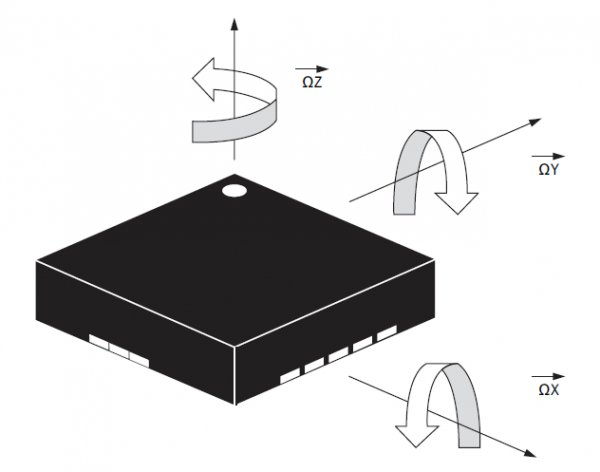
\includegraphics[width=0.5\textwidth]{img/gyroscope.jpg}
\caption{MEMS giroskopas, lenktos rodyklės atvaizduoja giroskopo išeities duomenis.}
\end{center}
\end{figure}

\subsection{Duomenų perdavimas}

Duomenų perdavimui naudojami berkeley TCP sockets tipo jungtis.
Startuodama "`Linux"' operacinės sistemos programa, atidaro serverio tipo TCP socket jungtį su porto numeriu 10001, ir laukia, kol bus atsiūstas prisijungimo prašymas.
Leidžiamas nedaugiau kaip vienas klientas vienu metu.
Prisijungęs prie serverio "`Android"' išmanusis telefonas pradeda siūsti matavimų duomenis. Matavimo duomenų paketas siunčiamas iškarto po kiekvieno atlikto matavimo.
Paketo formatas pavaizduotas pav. 2

\begin{figure}[H]
\begin{center}
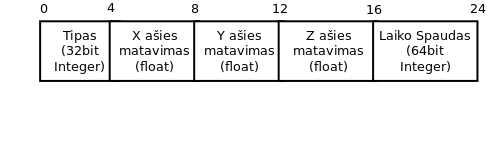
\includegraphics[width=0.6\textwidth]{img/packet.png}
\caption{Matavimo duomenų paketo formatas. Skaičiai parodo atstumą baitais nuo paketo pradžios.}
\end{center}
\end{figure}

Laukas "`tipas"' gali būti dviejų reiškmių: 
\begin{itemize}
	\item \textit{0} - Akselerometro duomenys (šiuo metu jie nėra naudojami "`Linux"' programoje)
	\item \textit{1} - Giroskopo duomenys
\end{itemize}

Laukai X, Y, Z ašims yra Akselerometro arba giroskopo matavimai. Kiekvienas skirtingas lauko "`tipas"' variantas išreiškia skirtingus matavimo vienetus:
\begin{itemize}
	\item Akselerometro - akseleracija visomis trimis ašimis išreikšta žemės gravitacijos lauko vienetais (g, $1g \approx 9,8 m/s^2$)
	\item Giroskopo - kampinis greitis visomis trimis ašimis išreikštas radianais per sekundę (rad/s)
\end{itemize}

Laiko spaudas naudojamas matavimų integracijai laiko atžvilgiu.
Integruojant reikia tiksliai žinoti kiek lako praėjo nuo vieno matavimo iki kito.
Verta paminėti, kad negalima pasitikėti duomenių gavimo momento laiku, nes interneto protokolai įveda didelius iškraipymus.

Laiko spaudas parodo kada buvo padarytas matavimas nanosekundėmis ($1ns = 10^{-9} s$) tam tikro (nežinomo, bet fiksuoto) taško laike atžvilgiu.
Šiuo atveju žinoti kieno atžvilgiu yra daromas laiko spaudas nėra reikalo, nes programos algoritmas suformuotas taip, kad dirbama tik su laiko skirtumais tarp matavimų.
Verta pastebėti, kad šioje vietoje negalima imti įprasto laiko (angliškai vadinamo "`wall clock"'), nes jis yra koreguojamas ir įvykus koregavimui, laiko skirtumas tarp matavimų nebeatspindės realaus prabėgusio laiko.
Įprastam mobiliajame telefone šie koregavimai įvyksta palyginus dažnai, todėl būtinai reikia operacinės sistemos užklausti nekoreguojamo laiko.


\subsection{Duomenų apdorojimas}

Šio darbo tikslas yra atvaizduoti realaus pasaulio trimačius sukamuosius judesius virtulioje aplinkoje.
Mūsų įeities duomenys yra sukamasis vektorius lokalioje (išmaniojo telefono) koordinačių sistemoje, tad tai reikia atvaizduoti į openGL modelio aplinką.
OpenGL aplinka pateikia funkcija glRotate, kuri leidžia pasukti objektą.
Jeigu į objekto matricą nėra užkraunama identity matrica, tuomet ši funkcija atvaizduoja pasukimą pagal krypties vektorių ir kampo didumą lokalioje to objekto koordinačių sistemoje.
Šiame algoritme, gavus naują duomenų paketą, gautas sukimo vektorius yra padauginamas iš konstantos normalizuojančios sukimo greičius ir išsaugomas į kampinio greičio registrą.
Kiekvieno kadro paišymo metu, objektas yra pasukamas tuo sukimo vektoriumi (žinoma konvertuojant į glRotate funkcijos reikalaujamą sukimo vektoriaus su atskiru kampu formatą).
Tokie veiksmai atitinka sukimo vektoriaus integraciją laiko atžvilgiu, o tai pagal fiziką išduoda kampinę poziciją.







\section{Esamos problemos ir galimi patobulinimai}

\subsection{Dreifavimas}
Dabartinėje programos versijoje naudojami tik giroskopo duomenys, integruojami laiko atžvilgiu.
Tai sukelia vadinamą dreifavimo (eng.: "`Drift"') problemą.
Dėl šios problemos, matavimo paklaidos laikui bėgant sumuojasi, ir nukrypsta nuo realios padėties.

Galimas sprendimas būtų panaudoti sensorių duomenų sintezę (eng.: "`sensor fusion"') ir įtraukti magnetometro, bei akselerometro matavimus į kampinės padėties matavimus.
Duomenų apjungimui galėtų būti panaudotas kalmano filtras, kuris leistų absoliučiai išvengti dreifavimo problemos.

\subsection{Žemas matavimų dažnis}
Mobilusis telefonas matavimus atlieka palyginus žemu dažniu, todėl greitai pakračius telefoną dreifavimo problema įveda katastrofiškas paklaidas.
Iš dalies šią problemą galėtų spręsti kalmano filtras ir "`sensor fusion"' algoritmas apibūdintas prieštai buvusioje posekcijoje, bet speciali techninė įranga su matavimo dažniu siekančiu 500-1000Hz leistų atlikti itin tikslius kampinės pozicijos matavimus.

\section{Išvados}

Šiame darbe yra pasiūlomas ir išbandomas integracinis metodas laisvai prienamų, išmaniuosiuose telefonuose montuojamų, MEMS giroskopų panaudojimui trimačių objektų manipuliacijai.
Dėja rezultatai rodo, kad vien integruojami giroskopo duomenys suteikia stiprų dreifavimą, ir patogiai trimačių objektų manipuliacijai būtina kompensuoti dreifavimą.



\end{document}



